\section{The Standard Model of Particle Physics}

The standard model (SM) of particle physics describes all of the known
particles and their interactions through the fundamental forces
(except for gravity): the strong nuclear force, the weak nuclear force, and the electromagnetic
force. These forces arise due to the exchange of spin-$1$
bosons among the spin-$\frac{1}{2}$ fermions that make up matter. The SM is a renormalizable quantum field
theory based on the gauge symmetry group $\mathrm{SU(3)}_{\mathrm{C}}\times \mathrm{SU(2)}_{\mathrm{L}}\times
\mathrm{U(1)}_Y$. Each factor in the gauge group corresponds to a fundamental force, represented by a gauge field, whose excitations are
the gauge bosons that act as force carriers:
\begin{center}
\begin{tabular}{ccccc}
$\mathrm{SU(3)}_{\mathrm{C}}$ &$\times$& $\mathrm{SU(2)}_{\mathrm{L}}$
  &$\times$& $\mathrm{U(1)}_Y$\\
 $\downarrow$&&$\downarrow$&&$\downarrow$\\
 $G_{\mu}^{\alpha}$&&$W^a_{\mu}$&&$B_{\mu}$\\
 $\alpha=1,...,8$&&$a=1,2,3$&&
\end{tabular}
\end{center}
The eight spin-$1$ bosons, $G_{\mu}^{\alpha}$,
associated with the factor $SU(3)_{\mathrm{C}}$ are the gluons. Any
particle that transforms is said to carry color charge. The three spin-$1$
bosons, $W^{a}_{\mu}$ are associated 

The matter fields are fermions, which fall into two
categories: the quarks, $u$, $d$, $c$, $s$, $t$, and $b$, which participate in the
strong interactions, and the leptons, $e$, $\mu$, $\tau$, $\nu_e$,
$\nu_{\mu}$, and $\nu_{\tau}$, which do
not. Fig.~\ref{fig:standardmodel} shows the particles in the SM. To simplify notation, it makes sense to consider the doublet of
$q_L = \binom{u_L}{d_L}$ and $\ell_L = \binom{e_L}{\nu_L}$. All matter fields implicity have
three-component generation indices $e_i=(e,\mu,\tau),
\nu_i=(\nu_e,\nu_{\mu},\nu_{\tau}), u_i=(u,c,t),
d_i=(d,s,b)$. 

The electric charge is given by $Q = T_{3L}+Y$.

Tab.~\ref{tab:representations} summarizes the
representations in which the fields transform under the SM
gauge group. The SM Langrangian
excluding Higgs and Yukawa terms is then,
\begin{align}
\mathcal{L}_{\mathrm{SM}} &= -\frac{1}{4}B_{\mu\nu}B^{\mu\nu} -\frac{1}{4}W^{a}_{\mu\nu}W^{a\mu\nu} - \frac{1}{4}G^{\alpha}_{\mu\nu}G^{\alpha\mu\nu}
  & \mathrm{(gauge~terms)}\nonumber\\
& +\bar\ell_L\tilde\sigma^{\mu}iD_{\mu}\ell_L +
   \bar e_R\sigma^{\mu}iD_{\mu}e_R + \bar v_R
   \sigma^{\mu}iD_{\mu}\nu_R + (\mathrm{h.c.})& \mathrm{(lepton~kinetic~terms)}\nonumber\\
& +\bar q_L\tilde\sigma^{\mu}iD_{\mu}q_L +
   \bar u_R\sigma^{\mu}iD_{\mu}u_R + \bar d_R
   \sigma^{\mu}iD_{\mu}d_R + (\mathrm{h.c.})& \mathrm{(quark~kinetic~terms)}\nonumber\\
& +\mathcal L_{\mathrm{Higgs}} +\mathcal L_{\mathrm{Yukawa}} &  \mathrm{(Higgs~and~Yukawa~terms)}
\label{eqn:lsm}
\end{align}

\begin{figure}
\centering
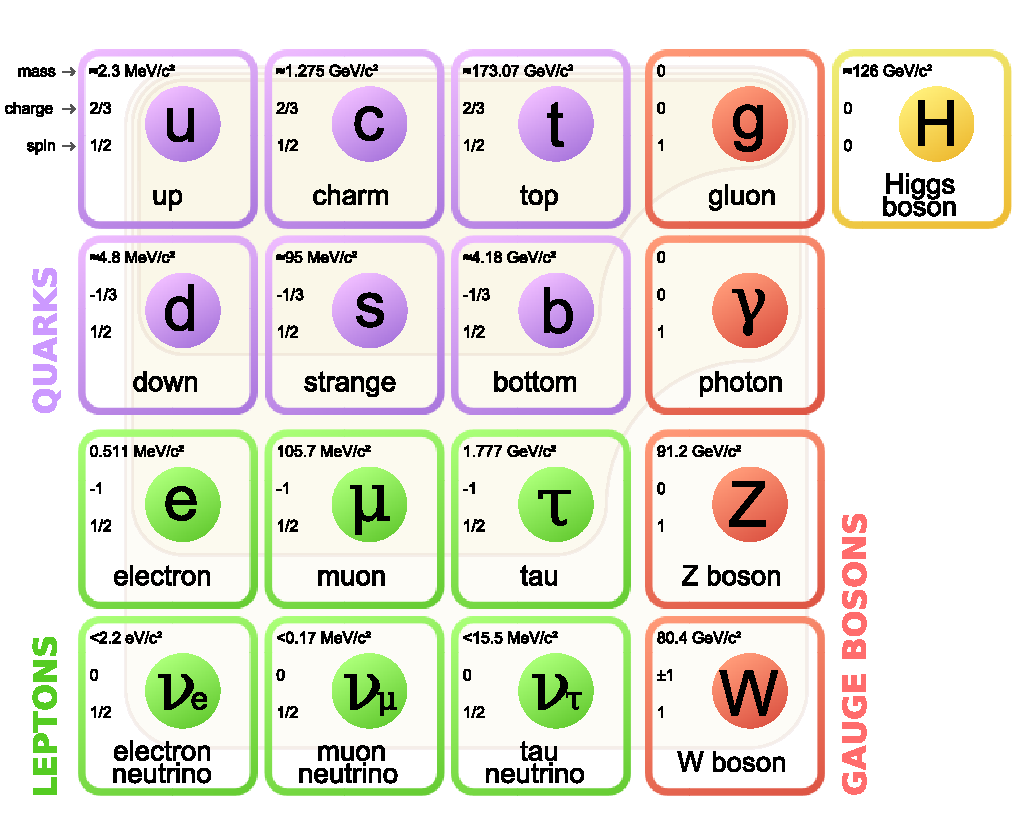
\includegraphics[width=0.7\textwidth]{figs/theory/standardmodel.pdf}
\caption{\label{fig:standardmodel} The particles in the standard model.}
\end{figure}

\begin{table}
\centering
\begin{tabular}{c|ccc}
&$\mathrm{SU(3)}_{\mathrm{C}}$&$\mathrm{SU(2)}_{\mathrm{L}}$&$\mathrm{U(1)}_Y$ \\
$q$ & $\mathbf{3}$ & $\mathbf{2}$ & $1/6$\\
$\bar u_R$ & $\mathbf{\bar 3}$ & $\mathbf{1}$ & $-2/3$\\
$\bar d_R$ & $\mathbf{\bar 3}$ & $\mathbf{1}$ & $1/3$\\
$\ell$ & $\mathbf{1}$ & $\mathbf{2}$ & $-1/2$\\
$\bar e_R$ & $\mathbf{1}$ & $\mathbf{1}$ & $1$\\\hline
$h$ & $\mathbf{1}$ & $\mathbf{2}$ & $1/2$
\end{tabular}
\caption{\label{tab:representations} Table summarizing the
    representations in which the fields transform under the standard
    model gauge group.}
\end{table}


\section{Electroweak Symmetry Breaking}
A central feature of gauge theories is that the gauge bosons are
massless due to the fact that the gauge symmetry forbids explicit mass
terms in the Lagrangian. In the SM, the mechanism of electroweak symmetry breaking
is a framework to keep the structure of gauge symmetry and
interactions at high energy, and still generate the observed masses
of the $\PW$ and $\PZ$ gauge bosons. The SM scalar potential is:
\begin{equation}
V(\Phi) = -m_h^2\Phi^{\dagger}\Phi + \lambda(\Phi^{\dagger}\Phi)^2~,
\end{equation}
where the Higgs field $\Phi$ is a self-interacting
$\mathrm{SU(2)}_{\mathrm{L}}$ complex doublet with weak hypercharge $Y=1/2$:
\begin{equation}
\Phi = \frac{1}{\sqrt{2}}\left(\begin{matrix} \sqrt{2}\phi^{+}\\\phi^0+ia^0\end{matrix} \right)~.
\end{equation}
If the quadratic term is negative, that is $m_h^2$ is positive, then
the minimum of the potential will occur at a value of of the Higgs
field that is not $\mathrm{SU(2)}_{\mathrm{L}}\times\mathrm{U(1)}_Y$ invariant.
We say the electroweak symmetry
$\mathrm{SU(2)}_{\mathrm{L}}\times\mathrm{U(1)}_Y$ is spontaneously
broken to $\mathrm{U(1)}_{\mathrm{EM}}$. Spontaneous symmetry breaking
is the phenomenon in which the equations of the dynamics are
exactly symmetric, but they admit solutions that are not.

\begin{equation}
\mathcal L_{\mathrm{Higgs}} = (D_{\mu}\Phi)^{\dagger}(D^{\mu}\Phi) - V(\Phi)
\end{equation}
\section{Higgs Mass and Naturalness}
The leading quantum correction to the Higgs mass squared parameter is due to
the large Yukawa coupling coupling to the top quark, which gives the
top quark its large mass,
\begin{fmffile}{higgs}
\begin{align}
\Delta(m^2_{h^0}) &= \quad\parbox{20mm}{
\begin{fmfgraph*}(20,20)
\fmfkeep{fermion}
\fmfleft{i} 
\fmfright{o} 
\fmf{dashes}{i,v1}
\fmf{dashes}{v2,o}
\fmf{plain,left,tension=.3,label=$t$}{v1,v2}
\fmf{plain,left,tension=.3}{v2,v1}
\fmfv{label=$h^0$,label.angle=90}{i}
\end{fmfgraph*}} \quad + \quad\cdots\\
&= -\frac{|\lambda_t|^2}{8\pi^2}\Lambda_{\mathrm{UV}}^2 + \cdots~,
\end{align}
where $\Lambda_{\mathrm{UV}}$ is an ultraviolet momentum cutoff.

\begin{align}
\Delta(m^2_{h^0}) &= \quad\parbox{20mm}{\fmfreuse{fermion}} \quad + \quad
\parbox{20mm}{
\begin{fmfgraph*}(20,20)
\fmfkeep{boson}
\fmfleft{i} 
\fmfright{o} 
\fmf{dashes}{i,v}
\fmf{dashes,right,tension=0.7,label=$\tilde t_{1,,2}$}{v,v}
\fmf{dashes}{v,o}
\fmfv{label=$h^0$,label.angle=90}{i}
\end{fmfgraph*}}
 \quad + \quad
\parbox{20mm}{
\begin{fmfgraph*}(20,20)
\fmfkeep{sunset}
\fmfleft{i}
\fmfright{o}
\fmf{dashes}{i,v1}
\fmf{dashes}{v2,o}
\fmf{dashes,left,tension=.3,label=$\tilde t_{1,,2}$}{v1,v2}
\fmf{dashes,left,tension=.3}{v2,v1}
\fmfv{label=$h^0$,label.angle=90}{i}
\end{fmfgraph*}} \quad + \quad\cdots\\
 &= -\frac{|\lambda_t|^2}{8\pi^2}\Lambda_{\mathrm{UV}}^2 +
  \sum_{i=1}^{2} \left ( \frac{\lambda_{\tilde
  t_i}^2}{16\pi^2}\Lambda_{\mathrm{UV}}^2 - 2m_{\tilde
  t_i}^2\log(\Lambda_{\mathrm{UV}}/m_{\tilde t_i}) \right )+ \cdots~,
\end{align}
\end{fmffile}

\section{Supersymmetry}
As shown by Coleman and Mandula, every local renormalizable quantum
field theory in four-dimensional Minkowski spacetime with
\begin{itemize}
\item finite number of different one-particle states
\item non-trivial interactions
\item mass gap
\end{itemize}
can only have a symmetry \emph{Lie algebra} of the S matrix which is a
direct product of the Poincar\'{e} group and an internal group.

However, this theorem has an infamous loophole in that it assumes the
symmetry algebra of the S matrix contains only commutators, but not
\emph{anticommutators} as a so-called \emph{Lie superalgrebra}
does. In particular, the Lie superalgebra for $\mathcal N=1$
supersymmetry is given in \ref{eqn:n1susy},

\begin{eqnarray}
~\{ Q_{\alpha},\bar Q_{\dot{\beta}}\} &=& 2\sigma^m_{\alpha\dot\beta} P_m \nonumber\\
~\{ Q_{\alpha},Q_{\beta}\} &=& \{ \bar Q_{\dot\alpha},\bar Q_{\dot\beta}\} = 0\nonumber\\
~[ P_m, Q_{\alpha}] &=& [P_m,\bar Q_{\dot\alpha}] = 0
\label{eqn:n1susy}
\end{eqnarray}

\subsection{Minimal Supersymmetric Standard Model}
The K\"{a}hler potential and super potential for chiral superfields
\begin{equation}
\mathcal L = \int d^4\theta K(\Phi,\Phi^{\dagger}) + \left (\int
  d^2\theta W(\Phi) + \mathrm{h.c.} \right)
\label{eqn:mssmlag}
\end{equation}

\begin{table}
\centering
\begin{tabular}{c|ccc}
&$\mathrm{SU(3)}_{\mathrm{C}}$&$\mathrm{SU(2)}_{\mathrm{L}}$&$\mathrm{U(1)}_Y$ \\
$Q$ & $\mathbf{3}$ & $\mathbf{2}$ & $1/6$\\
$U^c$ & $\mathbf{\bar 3}$ & $\mathbf{1}$ & $-2/3$\\
$D^c$ & $\mathbf{\bar 3}$ & $\mathbf{1}$ & $1/3$\\
$L$ & $\mathbf{1}$ & $\mathbf{2}$ & $-1/2$\\
$E^c$ & $\mathbf{1}$ & $\mathbf{1}$ & $1$\\\hline
$H_u$ & $\mathbf{1}$ & $\mathbf{2}$ & $1/2$\\
$H_d$ & $\mathbf{1}$ & $\mathbf{2}$ & $-1/2$
\end{tabular}
\caption{\label{tab:representations} Table summarizing the
    representations in which the superfields transform under the standard
    model gauge group.}
\end{table}

The R-parity conserving part of the superpotential is whown in Eqn.~\ref{eqn:Wrpc}
\begin{equation}
W_{\mathrm{RPC}} = - y_u H_u Q U^c + y_dH_d Q D^c + y_e H_d L E^c +
\mu H_uH_d
\label{eqn:Wrpc}
\end{equation}
while the R-partiy violating part is shown in \ref{eqn:Wrpv}
\begin{equation}
W_{\mathrm{RPV}} =\frac{1}{2}\lambda^{ijk}L_iL_jE_k^c +
\lambda^{\prime ijk} L_iQ_jD_k^c + \mu^{\prime i}H_uL_i +
\frac{1}{2}\lambda^{\prime\prime ijk}U_i^cD_j^cD_k^c
\label{eqn:Wrpv}
\end{equation}
From this we can write down the Lagrangian for the MSSM
\begin{equation}
\mathcal L_{\mathrm{MSSM}}=\frac{1}{2}\lambda^{ijk}L_iL_jE_k^c +
\lambda^{\prime ijk} L_iQ_jD_k^c + \mu^{\prime i}H_uL_i +
\frac{1}{2}\lambda^{\prime\prime ijk}U_i^cD_j^cD_k^c
\label{eqn:Wrpv}
\end{equation}



The mass matrices for the neutralinos and charginos are given by
\begin{equation}
\mathbf{M}_N =\left (  \begin{matrix}
M_1 & 0 & -m_Zs_Wc_{\beta} & m_Zs_Ws_{\beta} \\
0& M_2 & -m_Zc_Wc_{\beta} & -m_Zc_Ws_{\beta} \\
-m_Zs_Wc_{\beta}& m_zc_Wc_{\beta} & 0 & -\mu\\
m_Zs_Ws_{\beta}& -m_zc_Ws_{\beta} & \mu & 0
\end{matrix}\right)~,
\end{equation}
and 
\begin{equation}
\mathbf{M}_C =\left (  \begin{matrix}
M_2 & \sqrt{2}m_Ws_{\beta}\\
 \sqrt{2}m_Wc_{\beta}& \mu
\end{matrix}\right)~,
\end{equation}
respectively.
When the lightest neutralino is Higgsino-like ($\mu \ll M_1, M_2$), the
mass eigenvalues of the lightest neutralino, second lightest neutralino and chargino are close to
each other,
\begin{align}
m_{\chiz_1} &= \mu + \frac{m_Z^2(1+s_{\beta})(\mu - M_1c_W^2-M_2s_W^2)}{2(\mu-M_1)(\mu-M_2)} + \cdots\\
m_{\chiz_2} &= \mu + \frac{m_Z^2(1-s_{\beta})(\mu + M_1c_W^2+M_2s_W^2)}{2(\mu+M_1)(\mu+M_2)} + \cdots\\
m_{\chipm_1} &= \mu - \frac{m_W^2(\mu + M_2\sin 2\beta)}{M_2^2-\mu^2} + \cdots
\end{align}

Figure~\ref{fig:neutralinos} shows the mass differences
$m_{\chipm_1}-m_{\chiz_1}$ and $m_{\chiz_2}-m_{\chiz_1}$ as a function of the Wino mass $M_2$.


\begin{figure}[tb!]
\centering
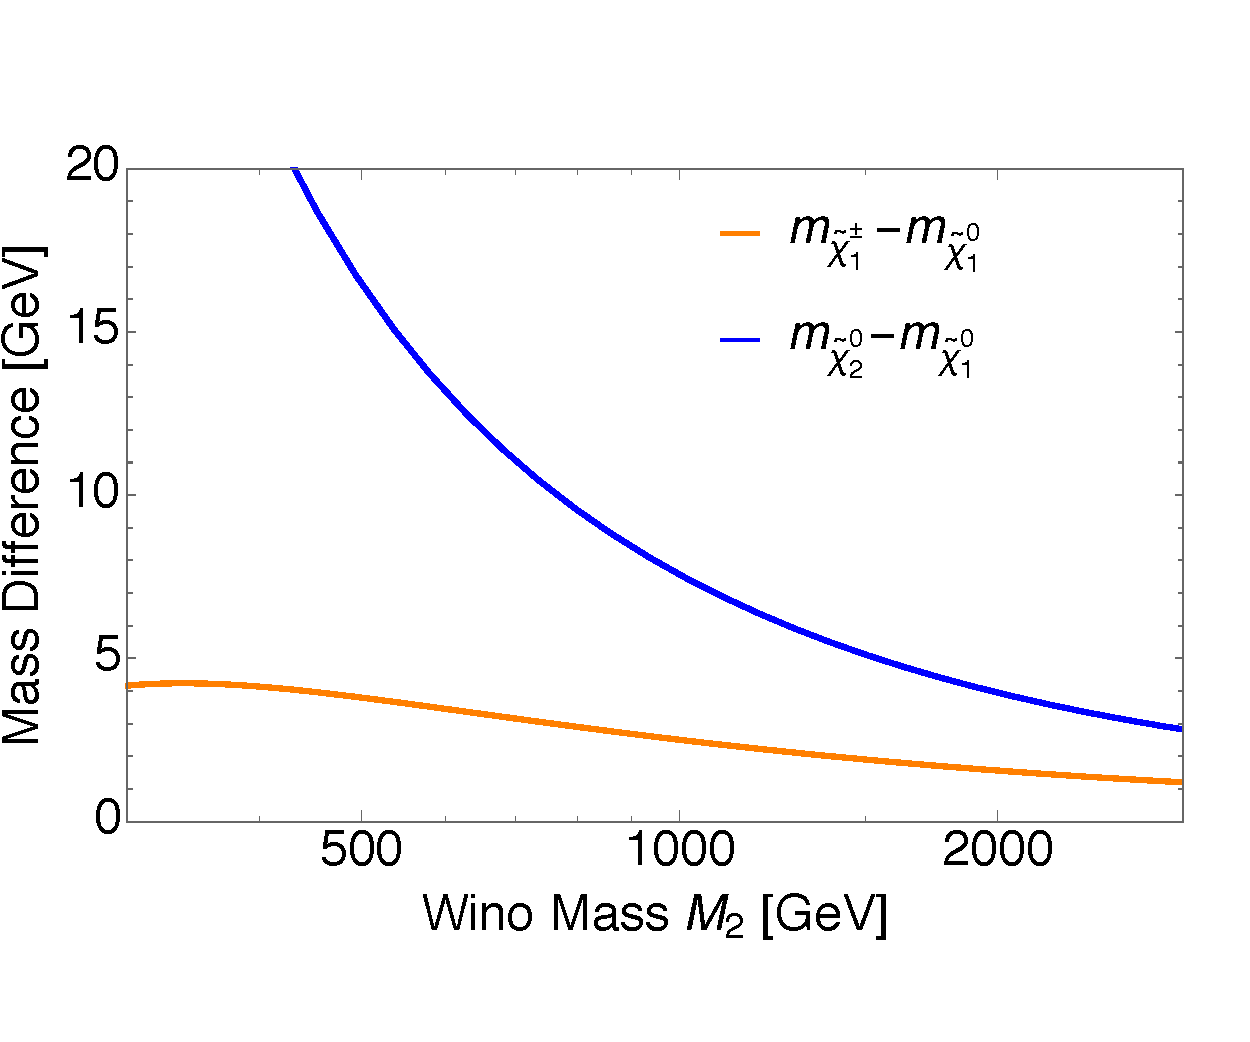
\includegraphics[width=0.8\textwidth,clip=true,viewport= 0 30 610 450]{figs/theory/neutralinos.pdf}
\caption{The mass difference between the lightest chargino and the
  lightest neutralino as a function of the Wino mass $M_2$
  assuming $\tan\beta=10$, $\mu=200 \GeV$ and $M_1 = 3 \TeV$.\label{fig:neutralinos}}
\end{figure}

\section{Simplified Natural Supersymmetry Models}
\label{sec:sms}

\begin{figure}[htb!]
\centering
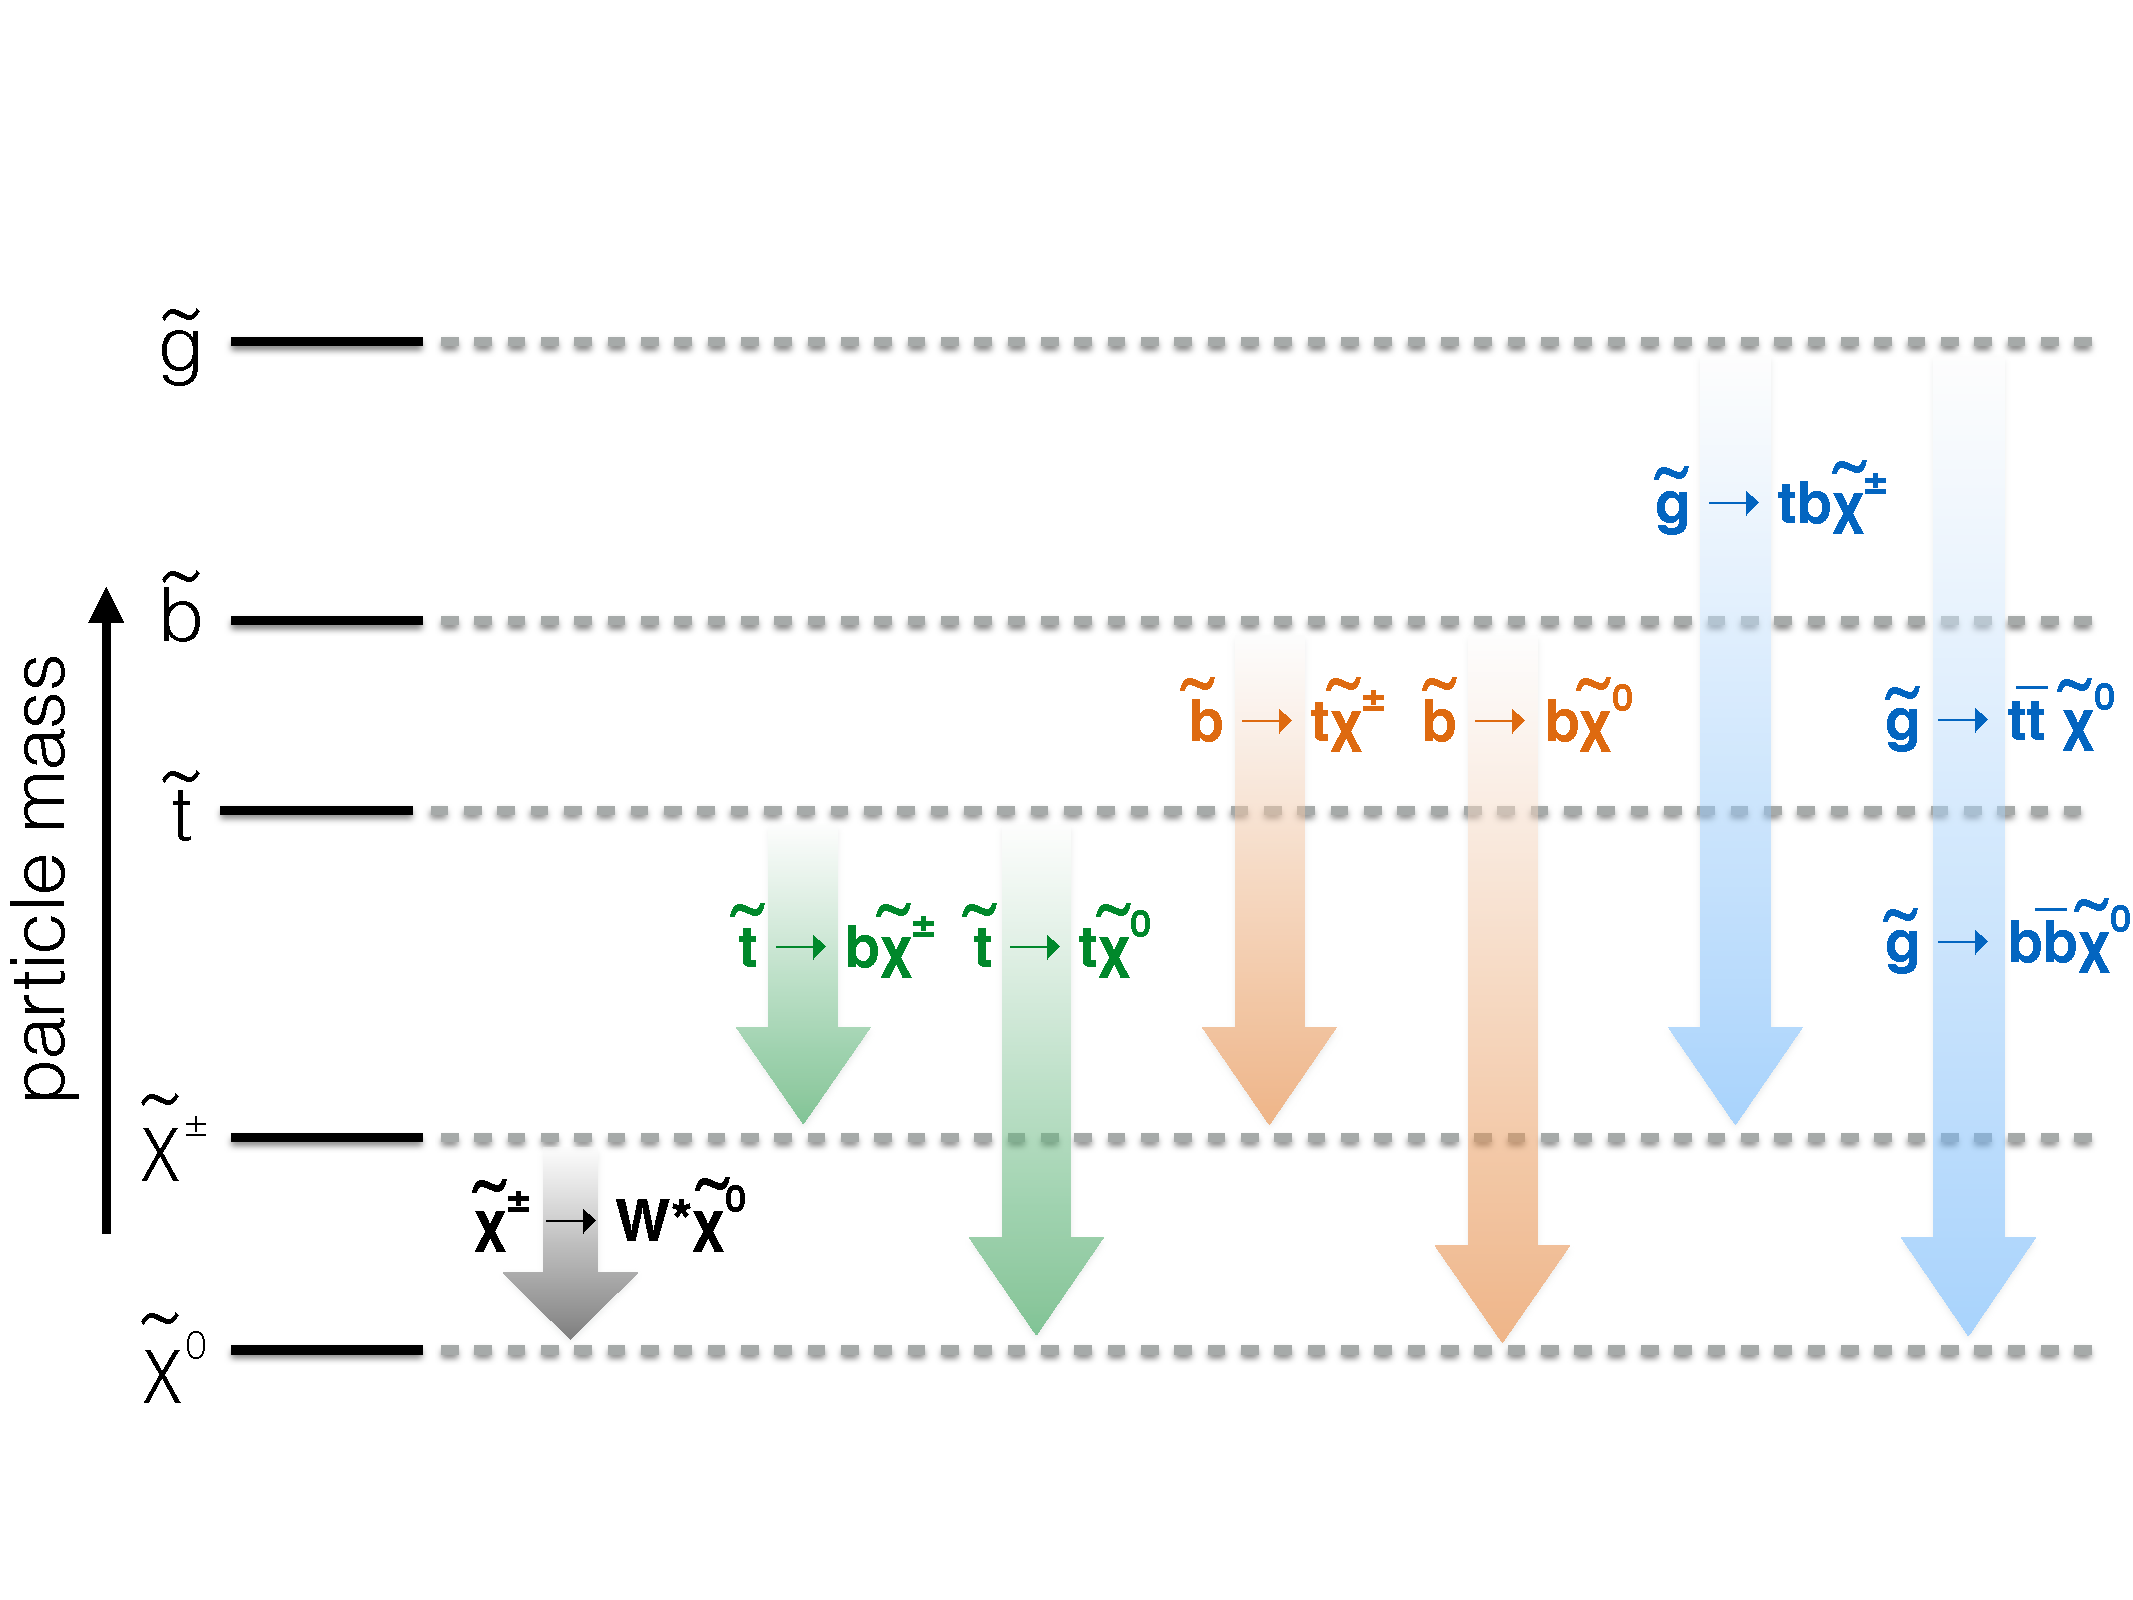
\includegraphics[width=0.85\textwidth]{figs/analysis8TeV/naturalSpectrum.pdf}
\caption{\label{fig:spectrum} The simplified natural SUSY spectrum
  considered in this paper, along with the assumed decay modes.}
\end{figure}

In Chapter~\ref{ch:analysis8TeV}, natural simplified SUSY scenarios are used to interpret
results. The LSP is the lightest neutralino $\chiz_1$ while the NLSP
is the lightest chargino $\chipm_1$.  They are both higgsinos and
their mass splitting is taken to be 5\GeV. The NLSP decays to the LSP
and a virtual $\PW$ boson ($\chipm_1 \to \PW^{\ast} \chiz_1$). The
other SUSY particles accessible at the LHC are the gluino and the
lightest top and bottom squarks. All other SUSY particles are
assumed to be too heavy to participate in the interactions. The SUSY
particles and their possible decay modes within this natural SUSY
spectrum are summarized in Fig.~\ref{fig:spectrum}.

In the context of this natural spectrum, several simplified
models~\cite{ArkaniHamed:2007fw,Alwall:2008ag,Alwall:2008va,Alves:2011sq,Alves:2011wf,Graesser:2012qy}
are considered for gluino pair production, based on three-body gluino
decays, in which each gluino decays to one of the following final states~\cite{SUS-11-016}:
\begin{itemize}
\item a top quark (antiquark) and a bottom antiquark (quark),
  and the NLSP; 
\item a top quark-antiquark ($\ttbar$) pair and the LSP;
\item a bottom quark-antiquark ($\bbbar$) pair and the LSP.
\end{itemize}
Furthermore, we separately consider the case in which each gluino
decays to
\begin{itemize}
\item a first or second generation quark-antiquark ($\qqbar$) pair and the LSP.
\end{itemize}
%\begin{itemize}
%\item \textbf{ T1bbbb}: pair-produced gluinos, each decaying with a 100\%
% branching fraction to a bottom quark-antiquark ($\bbbar$) pair and the LSP;
%\item \textbf{ T1tbbb}: pair-produced gluinos, each decaying with a
% 50\% branching fraction to a $\bbbar$ pair and the LSP or to a
 %top quark (antiquark), a bottom antiquark (quark), and the NLSP;
%\item \textbf{ T1ttbb}: pair-produced gluinos, decaying with a 100\%
%  branching fraction to a top quark (antiquark), a bottom antiquark
%  (quark), and the NLSP;
%\item \textbf{ T1tttb}: pair-produced gluinos, each decaying with a
% 50\% branching fraction to a top quark-antiquark ($\ttbar$) pair and the LSP or to a top
% quark (antiquark), a bottom antiquark (quark), and the NLSP;
%\item \textbf{ T1tttt}: pair-produced gluinos, each decaying with a 100\%
% branching fraction to a $\ttbar$ pair and the LSP.
%\end{itemize}
The corresponding Feynman diagrams are shown in
Fig.~\ref{fig:SMSGluinoTopology}.

\begin{figure*}[thb!]
\centering
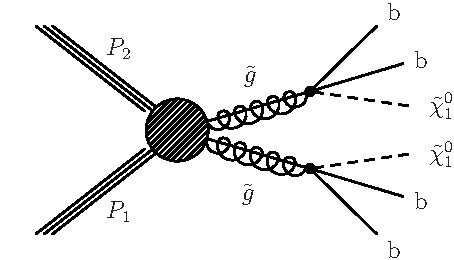
\includegraphics[width=0.32\textwidth]{figs/theory/T1bbbb.pdf}
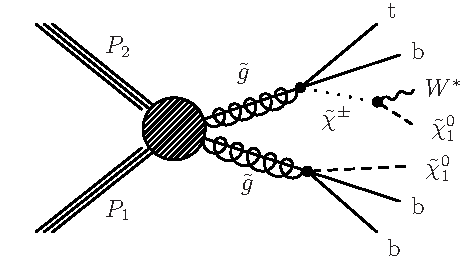
\includegraphics[width=0.32\textwidth]{figs/theory/T1tbbb.pdf}
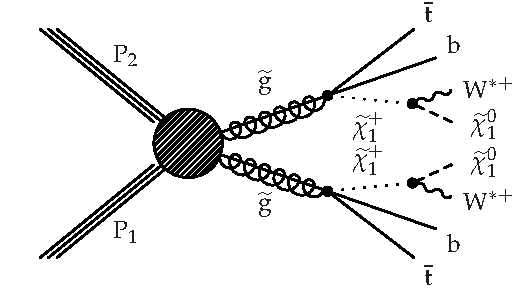
\includegraphics[width=0.32\textwidth]{figs/theory/T1ttbb.pdf} \\
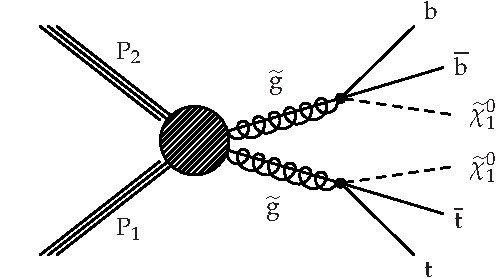
\includegraphics[width=0.32\textwidth]{figs/theory/T1tbtb.pdf} 
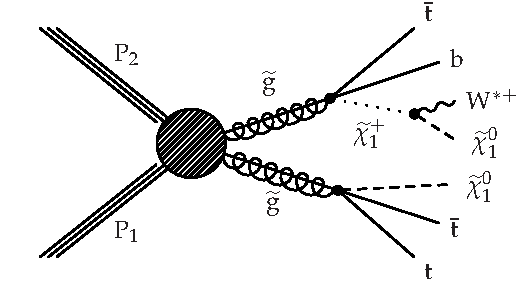
\includegraphics[width=0.32\textwidth]{figs/theory/T1tttb.pdf}
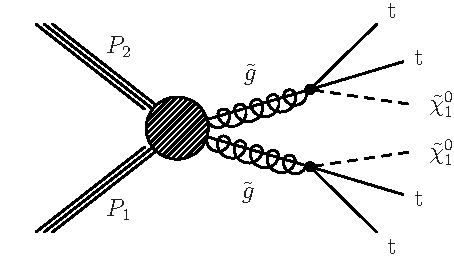
\includegraphics[width=0.32\textwidth]{figs/theory/T1tttt.pdf} \\
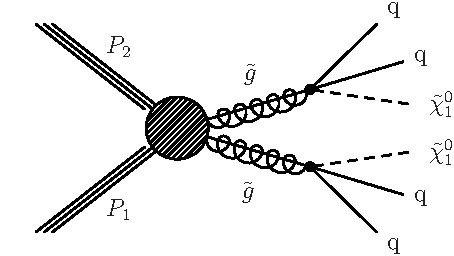
\includegraphics[width=0.32\textwidth]{figs/theory/T1qqqq.pdf} \\
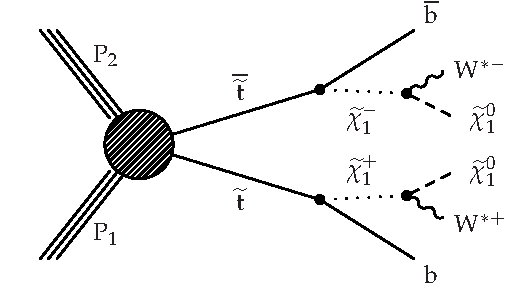
\includegraphics[width=0.32\textwidth]{figs/theory/T2bw.pdf}
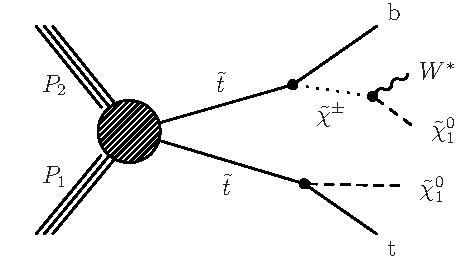
\includegraphics[width=0.32\textwidth]{figs/theory/T2tb.pdf}
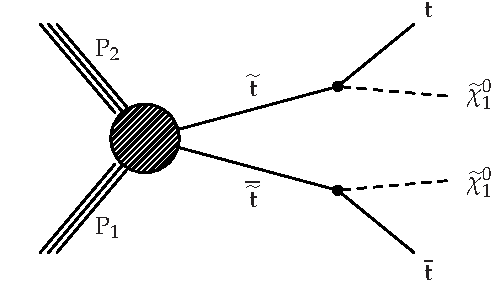
\includegraphics[width=0.32\textwidth]{figs/theory/T2tt.pdf}
\caption{Diagrams displaying the event topologies of gluino (upper 7
  diagrams) and top-squark (lower 3 diagrams) pair production
  considered in this thesis.\label{fig:SMSGluinoTopology}}
\end{figure*}


In addition, several simplified models are considered for
the production of top-squark pairs, in which each top squark decays to
one of the following final state:
 \begin{itemize}
\item a bottom quark and the NLSP;
\item a top quark and the LSP.
\end{itemize}
%\begin{itemize}
%\item \textbf{ T2bW$^{\ast}$}: pair-produced top squarks, each decaying
 % with a 100\% branching fraction to a bottom quark and the NLSP;
%\item \textbf{ T2tb}: pair-produced top squarks, each decaying with a 50\%
%  branching fraction to a top quark and the LSP or to a bottom quark and
%  the NLSP;
%\item \textbf{ T2tt}: pair-produced top squarks, each decaying with a
 % 100\% branching fraction to a top quark and the LSP.
%\end{itemize}
The corresponding Feynman diagrams are shown in
Fig.~\ref{fig:SMSGluinoTopology}.

\subsection{Technical Implentation in \PYTHIA}
To simplify the treatment of the sparticle decays in \PYTHIA v6.4.26, we directly implement three-body decays of
the form $\chipm_1 \to \chiz_1 f f^{\prime}$, with branching ratios
as shown in Table~\ref{tab:nlspbr}.
\begin{table}
\centering
\begin{tabular}{l|r}
decay mode & branching ratio \\\hline
$\chip_1 \to \chiz_1 u \bar d$ &  35.1\%\\
$\chip_1 \to \chiz_1 c \bar s$ &  35.1\%\\
$\chip_1 \to \chiz_1 e^+ \nu_e$ &  11.7\%\\
$\chip_1 \to \chiz_1 \mu^+ \nu_{\mu}$ &  11.7\%\\
$\chip_1 \to \chiz_1 \tau^+ \nu_{\tau}$ &  6.4\%
\end{tabular}
\caption{\label{tab:nlspbr}Table of branching ratios implemented in
  \PYTHIA v6.4.26 for the NLSP
  $\chipm_1$ in the simplified natural SUSY model considered in this chapter.}
\end{table}